% Usa o estilo abntex2, configurando detalhes de formatação e hifenização.
\documentclass[
	12pt,				
	oneside,		
	a4paper,			
	english,			% Idioma adicional para hifenização.
	french,				% Idioma adicional para hifenização.
	spanish,			% Idioma adicional para hifenização.
	brazil				% O último idioma é o principal do documento.
	]{abntex2}


%%% Importação de pacotes. %%%

% Pacotes não documentados:
\usepackage{etex}
\reserveinserts{28}
\usepackage{colortbl}
\usepackage{framed}

% Usa a fonte Latin Modern.
\usepackage{lmodern}

% Seleção de códigos de fonte.
\usepackage[T1]{fontenc}

% Codificação do documento em Unicode.
\usepackage[utf8]{inputenc}

% Usado pela ficha catalográfica.
\usepackage{lastpage}

% Indenta o primeiro parágrafo de cada seção.
\usepackage{indentfirst}

% Controle das cores.
\usepackage[usenames,dvipsnames]{xcolor}

% Permite usar o comando \hl{} para evidenciar texto com fundo amarelo. Útil para chamar atenção a itens a fazer.
% O comando \phl é definido para que o professor evidencie texto com uma cor diferente para adicionar notas.
\usepackage{soulutf8}
\newcommand{\phl}[2][Peach]{{\sethlcolor{#1} \hl{#2}}}

% Inclusão de gráficos.
\usepackage{graphicx}

% Inclusão de páginas em PDF diretamente no documento (para uso nos apêndices).
\usepackage{pdfpages}

% Para melhorias de justificação.
\usepackage{microtype}


% Citações padrão ABNT.
\usepackage[brazilian,hyperpageref]{backref}
\usepackage[alf]{abntex2cite}	
\renewcommand{\backrefpagesname}{Citado na(s) página(s):~}		% Usado sem a opção hyperpageref de backref.
\renewcommand{\backref}{}										% Texto padrão antes do número das páginas.
\renewcommand*{\backrefalt}[4]{									% Define os textos da citação.
	\ifcase #1
		Nenhuma citação no texto.
	\or
		Citado na página #2.
	\else
		Citado #1 vezes nas páginas #2.
	\fi}

% Pacotes não incluídos no template abntex2. 
% Podem ser comentados caso não queira utilizá-los.

% Inclusão de símbolos não padrão.
\usepackage{amssymb}
\usepackage{eurosym}

% Para utilizar \eqref para referenciar equações.
\usepackage{amsmath}

% Permite mostrar figuras muito largas em modo paisagem com \begin{sidewaysfigure} ao invés de \begin{figure}.
\usepackage{rotating}

% Permite customizar listas enumeradas/com marcadores.
\usepackage{enumitem}

% Permite inserir hiperlinks com \url{}.
\usepackage{bigfoot}
\usepackage{hyperref}

% Permite usar o comando \hl{} para evidenciar texto com fundo amarelo. Útil para chamar atenção a itens a fazer.
\usepackage{soul}

% Permite inserir espaço em branco condicional (incluído no texto final só se necessário) em macros.
\usepackage{xspace}

% Permite incluir listagens de código com o comando \lstinputlisting{}.
\usepackage{listings}
\usepackage{caption}
\DeclareCaptionFont{white}{\color{white}}
\DeclareCaptionFormat{listing}{\colorbox{gray}{\parbox{\textwidth}{#1#2#3}}}
\captionsetup[lstlisting]{format=listing,labelfont=white,textfont=white}
\renewcommand{\lstlistingname}{Listagem}
\definecolor{mygray}{rgb}{0.5,0.5,0.5}
\lstset{
	basicstyle=\scriptsize,
	breaklines=true,
	numbers=left,
	numbersep=5pt,
	numberstyle=\tiny\color{mygray}, 
	rulecolor=\color{black},
	showstringspaces=false,
	tabsize=2,
    inputencoding=utf8,
    extendedchars=true,
    literate=%
    {é}{{\'{e}}}1
    {è}{{\`{e}}}1
    {ê}{{\^{e}}}1
    {ë}{{\¨{e}}}1
    {É}{{\'{E}}}1
    {Ê}{{\^{E}}}1
    {û}{{\^{u}}}1
    {ù}{{\`{u}}}1
    {â}{{\^{a}}}1
    {à}{{\`{a}}}1
    {á}{{\'{a}}}1
    {ã}{{\~{a}}}1
    {Á}{{\'{A}}}1
    {Â}{{\^{A}}}1
    {Ã}{{\~{A}}}1
    {ç}{{\c{c}}}1
    {Ç}{{\c{C}}}1
    {õ}{{\~{o}}}1
    {ó}{{\'{o}}}1
    {ô}{{\^{o}}}1
    {Õ}{{\~{O}}}1
    {Ó}{{\'{O}}}1
    {Ô}{{\^{O}}}1
    {î}{{\^{i}}}1
    {Î}{{\^{I}}}1
    {í}{{\'{i}}}1
    {Í}{{\~{Í}}}1
}

% Colorinlistoftodos package: to insert colored comments so authors can collaborate on the content.
\usepackage[colorinlistoftodos, textwidth=20mm, textsize=footnotesize]{todonotes}
\newcommand{\bruno}[1]{\todo[author=\textbf{Bruno},color=green!30,caption={},inline]{#1}}
\newcommand{\vitor}[1]{\todo[author=\textbf{Vítor},color=red!30,caption={},inline]{#1}}




%%% Definição de variáveis. %%%

\renewcommand{\imprimircapa}{%
	\begin{capa}%
		\center
		
		{\ABNTEXchapterfont\large\subtitulo{}}
		\vfill
		\begin{center}
			\ABNTEXchapterfont\bfseries\LARGE\imprimirtitulo
		\end{center}
		
		\vfill
		Registro de Altera{\c c}{\~ o}es:
		\begin{table}[h]
			\centering
			\vspace{0.5cm}
			\begin{tabular}{|c|c|c|c|} \hline \rowcolor[rgb]{0.8,0.8,0.8}
			
 				Versão & Responsável & Data  & Alterações \\ \hline   
 				                            
				1.0  & \imprimirautor & 18/03/2016 & Versão inicial  \\ \hline 
				1.1  & Vítor E. Silva Souza & 05/04/2016 & Primeira revisão  \\ \hline 
				\versao{}  & \imprimirautor & 15/04/2016 & correções  \\ \hline 
				 
			\end{tabular}
		\end{table}
		
		\vfill
		\large\imprimirlocal
		\linebreak
		\large\imprimirdata
		\vspace*{1cm}
	\end{capa}
}


\newcommand{\versao}{1.2}
\newcommand{\subtitulo}{Documento de Projeto de Sistema}

\definecolor{lightgray}{gray}{0.9}

\titulo{SAE - Sistema de Acompanhamento de Egressos}
\autor{Bruno Manzoli do Nascimento}
\local{Vitória, ES}
\data{2015}

\instituicao{
  Universidade Federal do Espírito Santo -- UFES
  \par
  Centro Tecnológico
  \par
  Departamento de Informática}
\tipotrabalho{Monografia (PG)}







% Macros específicas do trabalho.
% (*) Inclua aqui termos que são utilizados muitas vezes e que demandam formatação especial.
% Os exemplos abaixo incluem i* (substituindo o asterisco por uma estrela) e Java com TM em superscript.
% Use sempre \xspace para que o LaTeX inclua espaço em branco após a macro somente quando necessário.
\newcommand{\istar}{\textit{i}$^\star$\xspace}
\newcommand{\java}{Java\texttrademark\xspace}
\newcommand{\latex}{\LaTeX\xspace}




%%% Configurações finais de aparência. %%%

% Altera o aspecto da cor azul.
\definecolor{blue}{RGB}{41,5,195}

% Informações do PDF.
\makeatletter
\hypersetup{
	pdftitle={\@title}, 
	pdfauthor={\@author},
	pdfsubject={\imprimirpreambulo},
	pdfcreator={LaTeX with abnTeX2},
	pdfkeywords={abnt}{latex}{abntex}{abntex2}{trabalho acadêmico}, 
	colorlinks=true,				% Colore os links (ao invés de usar caixas).
	linkcolor=blue,					% Cor dos links.
	citecolor=blue,					% Cor dos links na bibliografia.
	filecolor=magenta,				% Cor dos links de arquivo.
	urlcolor=blue,					% Cor das URLs.
	bookmarksdepth=4
}
\makeatother

% Espaçamentos entre linhas e parágrafos.
\setlength{\parindent}{1.3cm}
\setlength{\parskip}{0.2cm}



%%% Páginas iniciais do documento: capa, folha de rosto, ficha, resumo, tabelas, etc. %%%

% Compila o índice.
\makeindex




% Inicia o documento.
\begin{document}

% Retira espaço extra obsoleto entre as frases.
\frenchspacing


\begin{figure}[h]
  \centering
  
\includegraphics[scale=0.055]{figuras/brasao.jpg}
  \label{ppts3}
\end{figure} 

% Capa do trabalho.
\imprimircapa





%%% Início da parte de conteúdo do documento. %%%
% Marca o início dos elementos textuais.
\textual
% Inclusão dos capítulos.


\begingroup
\let\clearpage\relax
% ==============================================================================
% TCC - César Henrique Bernabé
% Capítulo 1 - Introdução
% ==============================================================================

\chapter{Introdução}
\label{sec-intro}

O avanço da tecnologia nas ultimas décadas permitiu que a complexidade das atividades realizadas por computadores se tornasse cada vez maior, demandando que projetos de sistemas de software passassem a abranger ainda mais os detalhes de domínio do ambiente em que os programas computacionais seriam executados ~\cite{andersson2009modeling,brun2009engineering}. Esse fator motivou estudos na área de modelagem e projeto de sistemas, fazendo com que novas pesquisas buscassem abranger os processos de projeto, construção e teste de software. 

Entretanto, para garantir a estabilidade dos sistemas, fazia-se uso majoritariamente da intervenção humana, o que rapidamente tornou-se inviável à medida que os sistemas cresciam para atender o aumento da demanda de novos usuários~\cite{andersson2009modeling}. Assim, a utilização de sistemas adaptativos vem tornando-se a solução mais viável e prática para a atual conjuntura do desenvolvimento de softwares. Além disso, o aumento do número de diferentes dispositivos e situações em que esses softwares podem ser executados faz com que eles passem a enfrentar uma grande diversidade de contextos (muitas vezes imprevisíveis) de execução, fundamentando ainda mais a pesquisa na área de softwares adaptativos~\cite{kephart2003vision}.

Sistemas adaptativos são dotados da capacidade de tomar decisões para se ajustar e se reconfigurar mediante mudanças de contexto, permitindo assim que os requisitos elicitados continuem a ser atendidos de forma satisfatória~\cite{souza2012requirement}. Entretanto, poucas soluções desse tipo consideram a modelagem das características adaptativas no sistema desde a fase de modelagem do mesmo. \zanshin~\cite{tesevitor} aparece como uma abordagem que baseia-se em modelos para projetar características adaptativas em sistemas por meio de novos tipos de requisitos, que definem o chamado ``ciclo de retroalimentação'', que operacionaliza a adaptação. Seguindo uma abordagem de Desenvolvimento Dirigido por Modelos, \zanshin apresenta um metamodelo que permite que modelos de sistemas sejam especificados de acordo com os requisitos do \framework.

Este trabalho encontra-se no contexto da pesquisa em torno da abordagem \zanshin, mais especificamente lidando com duas de suas limitações: (1) seu metamodelo atual não representa fielmente o conjunto de modelos desejados; e (2) não há uma ferramenta CASE que auxilie engenheiros de requisitos no uso da abordagem.



\section{Objetivos}
\label{sec-intro-objetivos}

Este trabalho possui dois objetivos principais: a reconstrução do metamodelo operacional do \zanshin e a criação de uma ferramenta gráfica usada para modelar sistemas adaptativos usando Engenharia de Requisitos Orientada a Objetivos (\textit{Goal-Oriented Requirements Engineering} ou \gore). O primeiro refere-se ao metamodelo de objetivos que é baseado em \textit{CORE} (\textit{Core Ontology for Requirements Engineering})~\cite{jureta2007core}, usado pelo framework para casar os requisitos do modelo de domínio específico com as instâncias dos elementos do metamodelo de \gore, e assim garantir que os objetivos do sistema estão sendo atendidos satisfatoriamente. Já a segunda atividade refere-se à ferramenta de modelagem de sistemas baseada nesse metamodelo operacional do \zanshin, usando sintaxe baseada em uma linguagem de especificação de modelos ontológicos conceituais conhecida como iStar~\cite{dalpiaz2016istar}. Para ambos os casos, foram utilizados os conceitos aprendidos ao longo do curso de Ciência da Computação. Dessa forma são objetivos específicos deste projeto:


\begin{itemize}
	
	\item Levantar as deficiências do metamodelo atual do \zanshin, identificando os pontos em que as relações entre os elementos deveriam ser modificadas para representarem mais fielmente as formalidades da Engenharia de Requisitos Orientada a Objetivos;
	
	\item Elaborar um metamodelo atualizado que, além de representar mais rigorosamente a hierarquia dos elementos \gore, também reflita as necessidades da arquitetura do \zanshin, como por exemplo as relações entre elementos;
	
	\item Modificar o código fonte do \textit{framework} para que o mesmo possa utilizar o novo metamodelo desenvolvido e executar o mecanismo de adaptações considerando esse novo metamodelo;
	
	\item Desenvolver uma ferramenta que permita ao usuário criar uma representação gráfica do modelo do sistema alvo e implementar, dentro dessa ferramenta, um módulo para converter o modelo gráfico representado para arquivos \xml que possam ser importados diretamente para o \zanshin;
	
	\item Apresentar os trabalhos desenvolvidos, juntamente com as perspectivas futuras de otimização de ambos os sistemas apresentados.

\end{itemize}


\section{Metodologia}
\label{sec-intro-metodologia}

O trabalho realizado compreendeu as seguintes atividades:


\begin{enumerate}
	
	\item \textit{Revisão Bibliográfica}: Estudo sobre Engenharia de Requisitos Orientada a Objetivos, Desenvolvimento Dirigido por Modelos e suas ferramentas, de publicações acadêmicas sobre \zanshin e sobre desenvolvimento de sistemas adaptativos;
	
	\item \textit{Estudo das Tecnologias:} Levantamento das tecnologias disponíveis para \textit{Eclipse Modeling Framework} (\emf) que permitam o desenvolvimento de editores gráficos dentro da plataforma \eclipse, de tecnologias que podem ser utilizadas para o desenvolvimento de editores gráficos e do código fonte do \zanshin (que também foi desenvolvido nessa plataforma);
	
	\item \textit{Elaboração do novo Metamodelo}: Nessa etapa o novo metamodelo a ser usado foi elaborado gradativamente a partir de informações obtidas dos documentos estudados e das discussões realizadas em reuniões com grupo de estudos de Engenharia de Requisitos na UFES;
	
	\item \textit{Adequação do \zanshin ao novo Metamodelo}: Após finalização do metamodelo, inicou-se processo de adequação do \framework para que o mesmo pudesse operar de acordo com a nova proposta, consistindo da modificação do código-fonte do \zanshin, bem como realização de testes de validação para garantir a consistência do novo metamodelo;
	
	\item \textit{Implementação da Ferramenta de Modelagem}: Uma primeira versão da ferramenta foi desenvolvida no contexto de trabalho de Iniciação Científica, entretanto a mesma usava o metamodelo antigo do \zanshin. Essa etapa consiste, portanto, no refatoramento da ferramenta gráfica que permite a modelagem de sistemas adaptativos seguindo as formalidades do novo metamodelo proposto para o sistema \zanshin, bem como a criação de módulo usando linguagem de transformação de modelos para texto, que permite a exportação do modelo desenvolvido nessa ferramenta para arquivo \xml adequado aos padrões do \framework;
	
	\item \textit{Redação da Monografia:} Escrita da monografia, etapa obrigatória do processo de elaboração do Projeto de Graduação. Para a escrita desta, foi utilizada a linguagem \textit{LaTeX}\footnote{LaTeX -- http://www.latex-project.org/} utilizando o template \textit{abnTeX}\footnote{abnTeX -- http://www.abntex.net.br} que atende os requisitos das normas da ABNT (Associação Brasileira de Normas Técnicas) para elaboração de documentos técnicos e científicos brasileiros. Para apoiar este processo, foi utilizado o aplicativo \textit{TeXstudio}.\footnote{www.texstudio.org}
	
\end{enumerate}


%%% Início de seção. %%%
\section{Organização do Texto}
\label{sec-intro-organizacao}

Este texto está dividido em quatro partes principais além desta introdução, que seguem:

\begin{itemize}
	\item \textbf{Capítulo \ref{sec-referencial} --} Referencial Teórico: apresenta discussão acerca de \gore e \mdd, focando na relação desses tópicos com sistemas adaptativos e com o processo de desenvolvimento da ferramenta \unagi. Ademais, é discutida a arquitetura do sistema \zanshin e suas características;
	
	\item \textbf{Capítulo \ref{sec-zanshin} --} Zanshin: nesse capitulo são apresentados os processos e decisões que levaram à elaboração do novo metamodelo do \zanshin, bem como as modificações decorrentes dessas modificações na arquitetura da plataforma;
	
	\item \textbf{Capítulo \ref{sec-unagi} --} Unagi: Nesse capítulo é abordado o processo de desenvolvimento da ferramenta \unagi e os pormenores da implementação de todos os módulos da mesma;
	
	\item \textbf{Capítulo \ref{sec-validacao} --} Revisão: é feita validação do metamodelo evoluído do \zanshin e da implementação da ferramenta \unagi;
	
	\item \textbf{Capítulo \ref{sec-conclusoes} --} Considerações Finais: apresenta as conclusões obtidas ao final deste trabalho, bem como as dificuldades encontradas e as perspectivas de trabalhos futuros para esse contexto.
\end{itemize}










\vspace*{2cm}

\endgroup

\chapter{ Plataforma de Desenvolvimento}
\label{sec-plataforma}



%=======================================================================================================
%			Tabela de Plataforma de Desenvolvimento e Tecnologias Utilizadas
%=======================================================================================================

Na Tabela~\ref{tabela-plataforma} são listadas as tecnologias utilizadas no desenvolvimento da ferramenta, bem como o propósito de sua utilização.

\begin{table}[h]
	\centering	
	\vspace{0.5cm}
	\footnotesize
	\begin{tabular}{|p{1.6cm}|c|p{5cm}|p{6.5cm}|}  \hline \rowcolor[rgb]{0.8,0.8,0.8}
	
 		Tecnologia & Versão & Descrição & Propósito \\\hline 
 		                             
		JavaEE & 7 & Conjunto de especificação de APIs e tecnologias, que são implementadas por programas servidores de aplicação. & Reduzir a complexidade do desenvolvimento, implantação e gerenciamento de aplicações, de modo que o desenvolvedor não se preocupe demasiadamente com segurança, escalabilidade e desempenho. \\ \hline
	
		Java & 8 & Linguagem de programação orientada a objetos e independente de plataforma. & Desenvolvimento de aplicativos em linguagem de programação orientada a objetos e independente de plataforma. \\\hline
		
		JSF & 2.2 & Framework web baseado em Java que tem como objetivo simplificar o desenvolvimento de interfaces de sistemas para a web. & Melhorar a produtividade, permitindo a construção de interfaces para web usando um conjunto de componentes pré-construídos, ao invés de criar interfaces inteiramente do zero.  \\\hline  
		 
		EJB & 3.2 & Componente da  plataforma JEE  que roda em um container de um servidor de aplicação.   &  Fornecer um desenvolvimento rápido e simplificado de aplicações Java, com base em componentes distribuídos, transacionais, seguros e portáveis.  \\\hline
		 
		JPA &  2.1  &   API para persistência de dados por meio de mapeamento objeto-relacional.  & Eliminar muito do trabalho com queries SQL e facilitar a manuntenção visto que menos linhas de código são necessárias.\\\hline
		
		CDI & 1.1  & API para injeção de dependências.   & Integração das diferentes camadas da arquitetura e serviços de transação. \\\hline
		
		JAAS & & Serviço de Autenticação e Autorização do Java & Controlar o acesso aos recursos do sistema    \\\hline
		
		AdminLTE & 2.3.0 & Template Bootstrap 3 resposivo &  Utilizar um tamplate responsivo open source que seja facilmente personalizado, engloba scripts	JS e folhas de estilos CSS para prover um layout responsivo além de muitos outros plugins.  \\\hline
		
		Facelets & 2.0 &  Sistema de template Web de código aberto.  & Reusar estrutura comum às paginas e facilitar futura manutenção do padrão visual do sistema.  \\\hline
		 
		  PrimeFaces & 5.1 &  Conjunto de componentes JSF open source com várias extensões.  & Reutilizar componentes avançados de interface gráfica.  \\\hline
		  
		MySQL Server &  5.6.23  & Sistema Gerenciador de Banco de Dados Relacional gratuito.    &  Persistência dos dados manipulados pela ferramenta.  \\\hline
		
		WildFly & 9.0.2 &  Servidor de Aplicações para Java EE. &  Prover acesso a aplicações web por meio do protocolo HTTP (HyperText Transfer Protocol). \\\hline
		
		
		
		
		% Hibernate \vitor{Não precisa. Você vai usar JPA e aceitar a implementação que vier no servidor de aplicações, certo? Não precisa mencionar o Hibernate.} & 4.3  &  Framework de mapeamento objeto-relacional gratuito que implementa a JPA.  &  Fazer mapeamento objeto-relacional.  \\\hline
		                              
	\end{tabular}
	\caption{Plataforma de Desenvolvimento e Tecnologias Utilizadas}	
	\label{tabela-plataforma}
\end{table}






%=======================================================================================================
%			Tabela de Softwares de Apoio ao Desenvolvimento do Projeto
%=======================================================================================================

\newpage
Na Tabela~\ref{tabela-software} vemos os softwares que apoiaram o desenvolvimento de documentos e também do código fonte.

\begin{table}[h]
	\centering	
	\vspace{0.5cm}
	\begin{tabular}{|p{3cm}|c|p{5cm}|p{6cm}|}  \hline \rowcolor[rgb]{0.8,0.8,0.8}
	
 		Tecnologia & Versão & Descrição & Propósito \\\hline 
 		 
		Eclipse Java EE IDE for Web Developers  & 4.5.1 & Ambiente de desenvolvimento (IDE) para a linguagem Java.  &	Facilitar a atividade de implementação de software.	  \\\hline 
 		                            
		Astah Community & 6.9.0 & Ferramenta para modelagem em UML & Ferramenta de modelagem UML (Unified Modeling Language). \\\hline
			              
		Apache Maven    & 3.2.5 & Ferramenta de gerência de projeto baseada em project object model (POM).  &  Simplificar o download das dependências do projeto.  \\\hline 
		
		Texmaker   & 4.1-1 &  Editor de LaTeX.  &  Desenvolver os Documentos necessários para o sistema.  \\\hline       
			              
	\end{tabular}
	\caption{Softwares de Apoio ao Desenvolvimento do Projeto}	
	\label{tabela-software}
\end{table}



\chapter{Atributos de Qualidade e Táticas}
\label{sec-atributos}

Na Tabela~\ref{tabela-atributos} são listados os atributos de qualidade considerados neste projeto, com uma indicação se os mesmos são condutores da arquitetura ou não e as táticas a serem utilizadas para tratá-los.


\begin{table}[h]
	\centering	
	\vspace{0.5cm}
	\begin{tabular}{|p{2.5cm}|p{2cm}|p{1.9cm}|p{8.4cm}|}  \hline \rowcolor[rgb]{0.8,0.8,0.8}
	
 		Categoria & Requisitos Não Funcionais & Condutor da Arquitetura & Tática \\\hline 
 		 
 		    
 		{} & {} & {} & 1- Organizar a arquitetura da ferramenta segundo uma combinação de camadas e partições.   \\
 		
 		Portabilidade & RNF-1 & Sim  & 2- A camada de lógica de negócio deve ser organizada segundo o padrão Camada de Serviço. \\
 		
		{} & {} & {} & 3- A camada de gerência de dados deve ser organizada segundo o padrão DAO. \\
 		  		
 		
 		{} & {} & {} & 4- Utilizar uma linguagem que seja compatível com os principais navegadores do mercado. \\ \hline  
 		  
 		                             
		Facilidade de Aprendizado, Facilidade de Operação & RNF-2, RNF-3 & Sim  & Prover ao usuário a capacidade de entrar com comandos que permitam operar o sistema de modo mais amigáveis. Para tal, as interfaces do sistema devem permitir, sempre que possível, a entrada por meio de seleção ao invés da digitação de campos. \\\hline
		
		
		Segurança de Acesso  & RNF-4 & Sim  & Identificar usuários usando login e autenticá-los por meio de senha. \\\hline
		  
		
		Eficiência em relação ao tempo & RNF-5 & Sim  & Utilizar campos de seleção ao invés de digitação. Uso de AJAX para uma interação mais eficiente entre usuário e sistema Web. \\\hline
	
	
		Interoperabi- lidade & RNF-6 & Sim  & Utilizacao da API Commons Mail. \\\hline 
		
		
		Reusabilidade & RNF-7 & Sim  & Reutilizar componentes e frameworks existentes. No caso, foi reutilizado o nemo-utils. Quando não houver componentes disponíveis e houver potencial para reúso, devem-se desenvolver novos componentes para reúso. \\\hline  
 		 
		                              
	\end{tabular}
	\caption{Atributos de Qualidade e Táticas Utilizadas}	
	\label{tabela-atributos}
\end{table}




\chapter{Arquitetura de Software}
\label{sec-arquitetura}

Antes de falar da arquitetura cabe destacar que o \imprimirtitulo, será implementado como módulos do Marvin, que é  um Sistema de Informação baseado na Web que agrega ferramentas úteis para o gerenciamento de tarefas de ensino e pesquisa em uma universidade.
Muitos estudantes do DI/Ufes desenvolve ferramentas como parte de seu projeto final de graduação assim o Marvin é uma tentativa de integrar essas ferramentas de uma forma que pode ser realmente usado por pessoas.

A arquitetura de software do sistema SAE, baseia-se na combinação de camadas e módulos. Cada um desses módulos, por sua vez, está organizado em três camadas seguindo o proposto pelo FrameWeb, a saber: Camada de Apresentação (\textit{Presentation Tier}), Camada de Negócios (\textit{Business Tier}) e Camada de Acesso a Dados (\textit{Data Access Tier}). De forma a dar suporte para a construção da aplicação, a ferramenta de apoio nemo-utils será utilizada. Tal ferramenta provê classes que auxiliam na implementação dos casos de uso cadastrais que seguem o modelo de arquitetura a ser utilizado.


A primeira camada contém os pacotes de Visão (\textit{View}) e Controle (\textit{Control}), a segunda contém o de Domínio (\textit{Domain}) e o de Aplicação (\textit{Application}) e a terceira somente o pacote de Persistência (\textit{Persistence}). Cada pacote será explicado melhor nas próximas seções onde serão descritos os dois módulos do SAE (\textit{Core} e \textit{Public}). A Figura~\ref{figura-arquitetura} apresenta a visão geral das camadas e seus pacotes juntamente com o relacionamento que existe entre eles e as tecnologias Java EE utilizadas em cada pacote.



\begin{figure}[h]
  \centering
  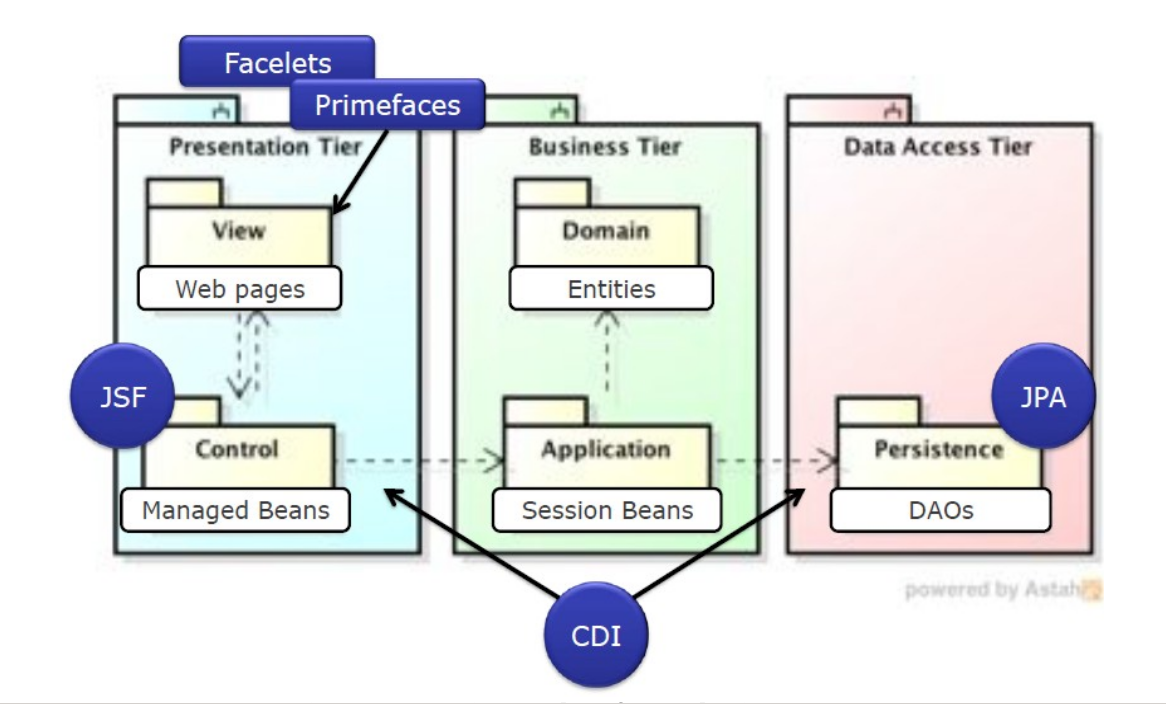
\includegraphics[width=0.9\textwidth]{figuras/arquitetura.png}
  \caption{Arquitetura de Software do Sistema~\cite{lima-pg15}}
  \label{figura-arquitetura}
\end{figure} 



A Figura~\ref{figura-modulos} apresenta a subdivisão de cada módulo nas camadas descritas acima, a saber a Camada de Apresentação (\texttt{control}), Camada de Negócios (\texttt{domain} e \texttt{application}) e Camada de Acesso a Dados (\texttt{persistence}).



\begin{figure}[h]
  \centering
  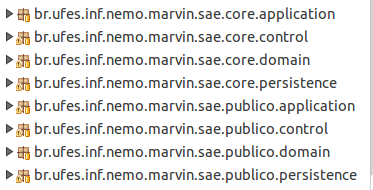
\includegraphics[scale=0.6]{figuras/modulos.png}
  \caption{Subdivisão dos módulos \texttt{sae.core} e \texttt{sae.public} de acordo com a arquitetura de software.}
  \label{figura-modulos}
\end{figure} 





%===================================================================================================================
%									Camada de Apresentação
%===================================================================================================================
\section{Camada de Apresentação}

As funcionalidades criar, visualizar, editar e excluir (abreviadas de CRUD, do inglês \textit{create, read, update and delete}), seguem um mesmo fluxo de execução e de interação com o usuário. Tais funcionalidades são similares para todos os casos de uso cadastrais devido a utilização da ferramenta nemo-utils. Esse fluxo de execução similar é representado na Figura~\ref{figura-modelo-view-crud} através de um modelo de apresentação genérico.

\begin{figure}[h]
  \centering
  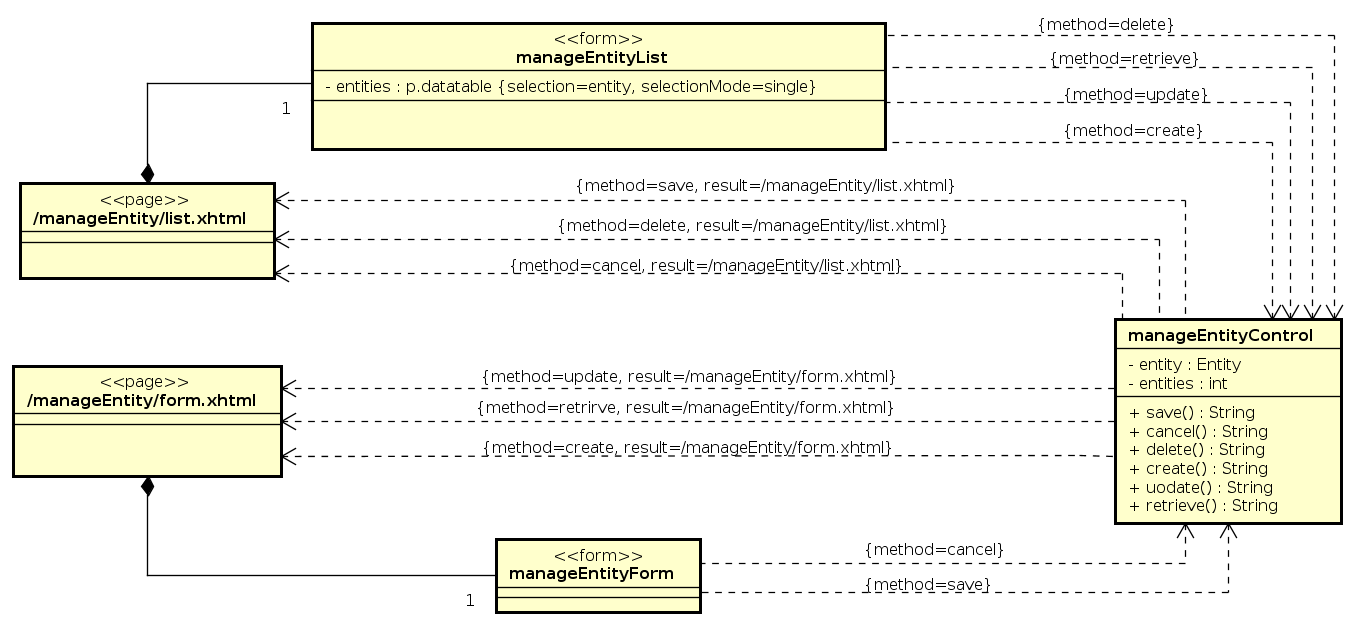
\includegraphics[width=1\textwidth]{figuras/modelocrud}
  \caption{Modelo de Navegação de um CRUD nemo-utils, usado como base para funcionalidades dos cadastros do sistema SAE~\cite{lima-pg15}.}
  \label{figura-modelo-view-crud}
\end{figure} 


Para os casos de uso que apresentam funções diferentes de apenas as básicas de cadastro, o modelo de navegação mostrado anteriormente não pode ser aplicado. Segue na Figura~\ref{figura-modelo-view-analisar-depoimento} o modelo de navegação para o fluxo \emph{Avaliar Depoimento} do caso de uso \emph{Gerenciar Depoimentos}, e na Figura~\ref{figura-modelo-view-consultar-depoimento} o modelo de navegação para o caso de uso \emph{Consultar Depoimentos}.

\begin{figure}[h]
  \centering
  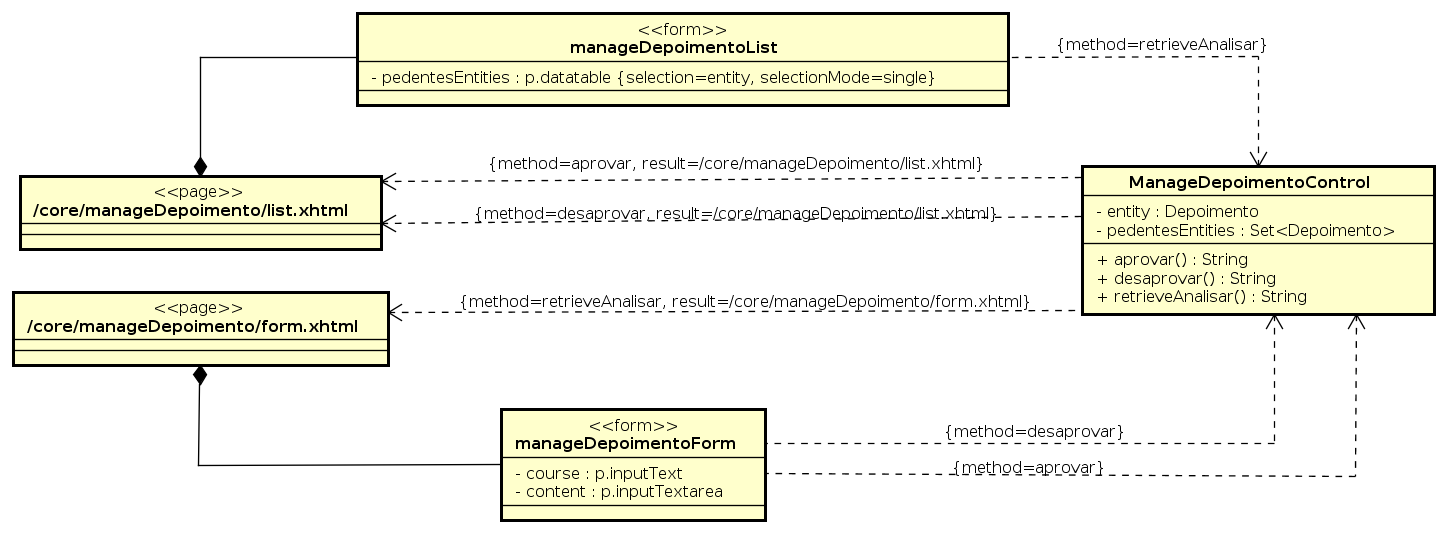
\includegraphics[width=1\textwidth]{figuras/analisarDepoimento}
  \caption{Modelo de Navegação - Avaliar Depoimento.}
  \label{figura-modelo-view-analisar-depoimento}
\end{figure}

\begin{figure}[h]
  \centering
  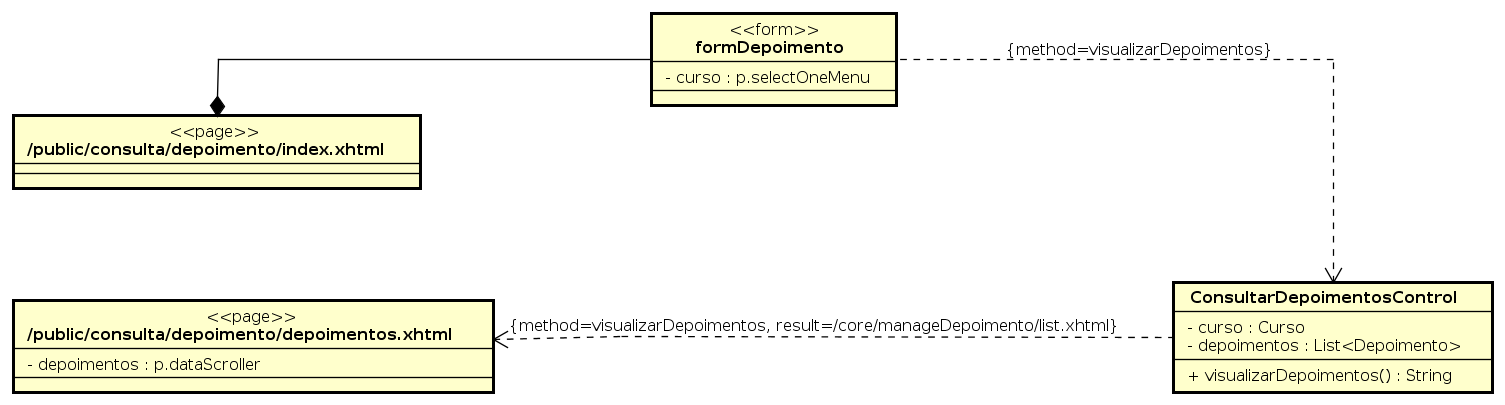
\includegraphics[width=1\textwidth]{figuras/consultarDepoimento}
  \caption{Modelo de Navegação - Consultar Depoimento.}
  \label{figura-modelo-view-consultar-depoimento}
\end{figure} 



%===================================================================================================================
%									Camada de Negócios
%===================================================================================================================
\section{Camada de Negócios }

\subsection{Dominio}
Diferente da abordagem original do FrameWeb original proposto em 2007, todos os atributos que são não nulos tiveram a \textit{tag} \texttt{not null} omitida e os que são nulos tiveram a tag \texttt{null} acrescida de forma a diminuir a poluição visual com repetições desnecessárias no diagrama.

Todas as classes de domínio estendem \texttt{PersistentObjectSupport} do pacote nemo-utils, sendo que essa herança não é mostrada nos diagramas com o intuito de não poluí-los com várias associações.

A Figura~\ref{figura-modelo-dominio-core} mostra o Modelo de Domínio para o módulo \textit{sae.core} e na Figura~\ref{figura-modelo-dominio-publico} o modelo de domínio para o módulo \textit{sae.public}.

\begin{figure}[h]
  \centering
  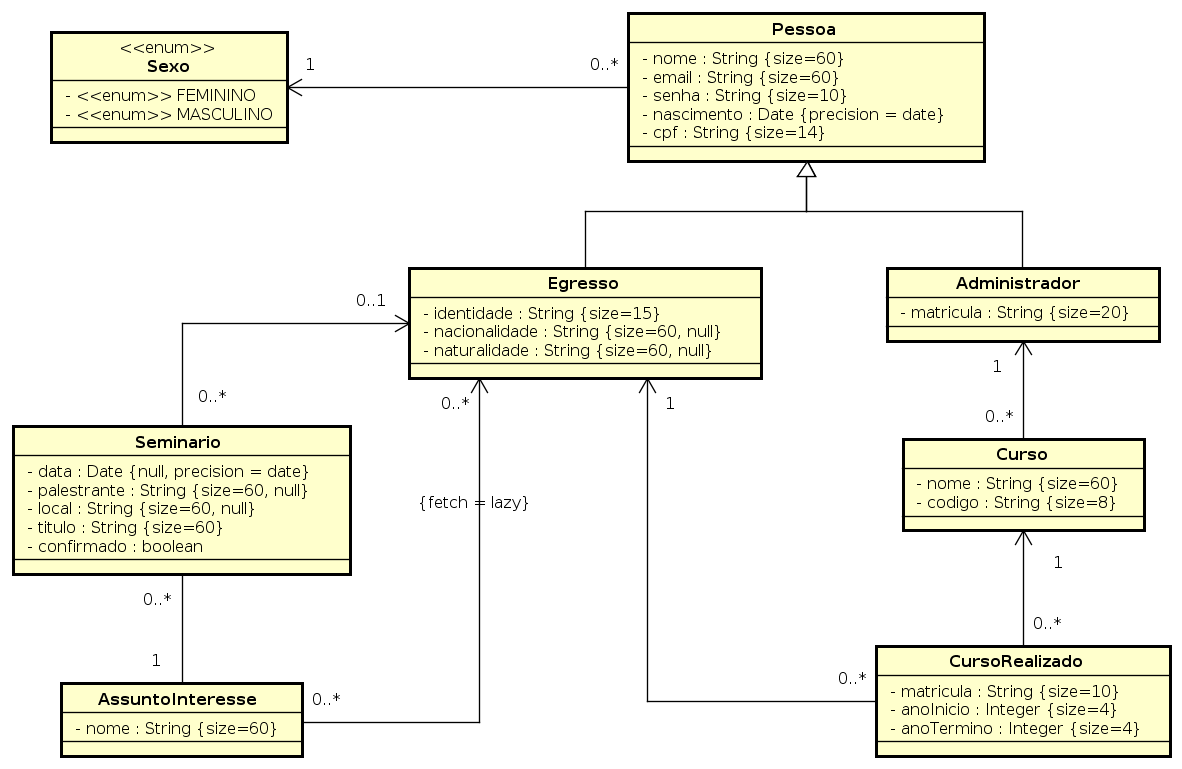
\includegraphics[width=1\textwidth]{figuras/fig-projeto-core-modelo-dominio}
  \caption{Modelo de Domínio do SAE para o módulo \textit{sae.core}.}
  \label{figura-modelo-dominio-core}
\end{figure} 
	
	
\begin{figure}[!h]
  \centering
  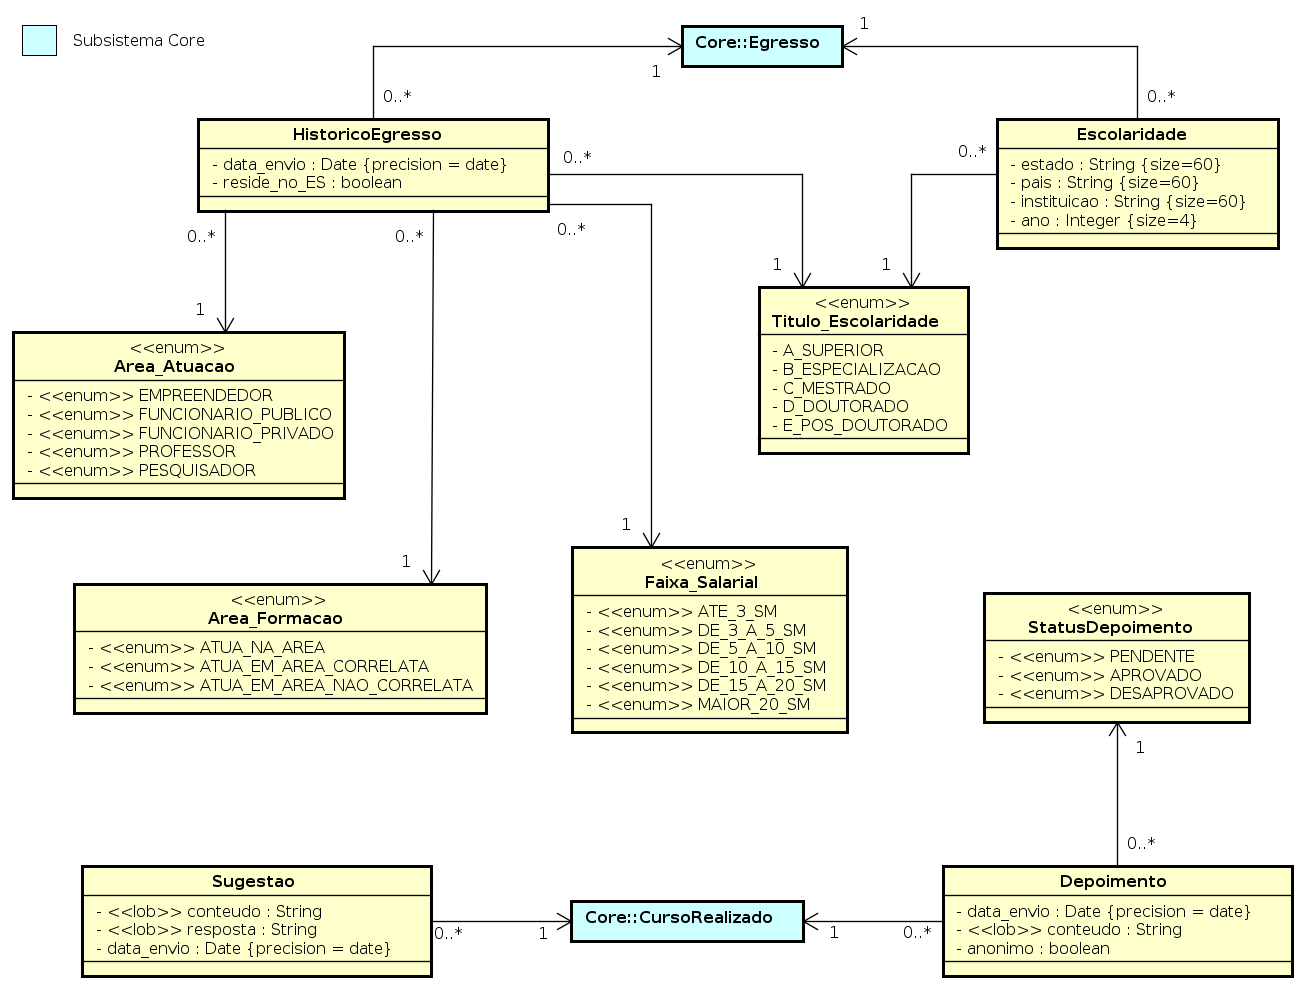
\includegraphics[width=1\textwidth]{figuras/modelodominiopublico.png}
  \caption{Modelo de Domínio do SAE para o módulo \textit{sae.public}.}
  \label{figura-modelo-dominio-publico}
\end{figure} 



Uma observação a ser feita é que classes com potencial de ser comuns a todos os módulos a serem desenvolvidos farão parte do pacote core do Marvin, assim as classes Administrador, Egresso e Curso farão parte deste pacote.







\newpage
\subsection{Aplicação}
Todas as classes de aplicação que são de casos de uso cadastrais estendem de \texttt{CrudServiceBean} do pacote nemo-utils, porém com uma pequena alteração, foi adicionado a classe uma anotação \texttt{@PermitAll} para poder realizar o controle de segurança, tal classe está representada na Figura~\ref{figura-modelo-aplicacao-generico} de forma genérica. Da mesma forma dos diagramas anteriores essa herança não é mostrada no diagrama com o intuito de não poluir o diagrama com várias associações. 

Os casos de uso não cadastrais Confirmar Seminário e Convidar Palestrante, devido sua baixa complexidade e sua alta relação com o caso de uso gereciar seminário, foram adicionados dentro de \texttt{ManageSeminario}.

\begin{figure}[!h]
  \centering
  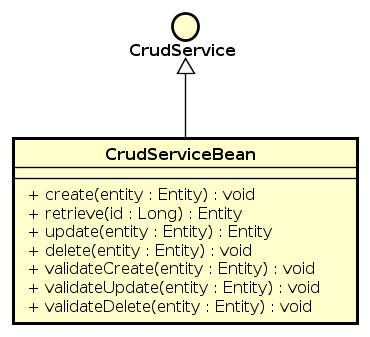
\includegraphics[scale=0.45]{figuras/crudservicebean.png}
  \caption{Modelo de Aplicação genérica da ferramenta nemo-utils.}
  \label{figura-modelo-aplicacao-generico}
\end{figure}

A Figura~\ref{figura-modelo-aplicacao-core} mostra o modelo de aplicação para o módulo \textit{sae.core} e a Figura~\ref{figura-modelo-aplicacao-publico} representa o modelo de aplicação para o módulo \textit{sae.public}.

\newpage

\begin{figure}[!h]
  \centering
  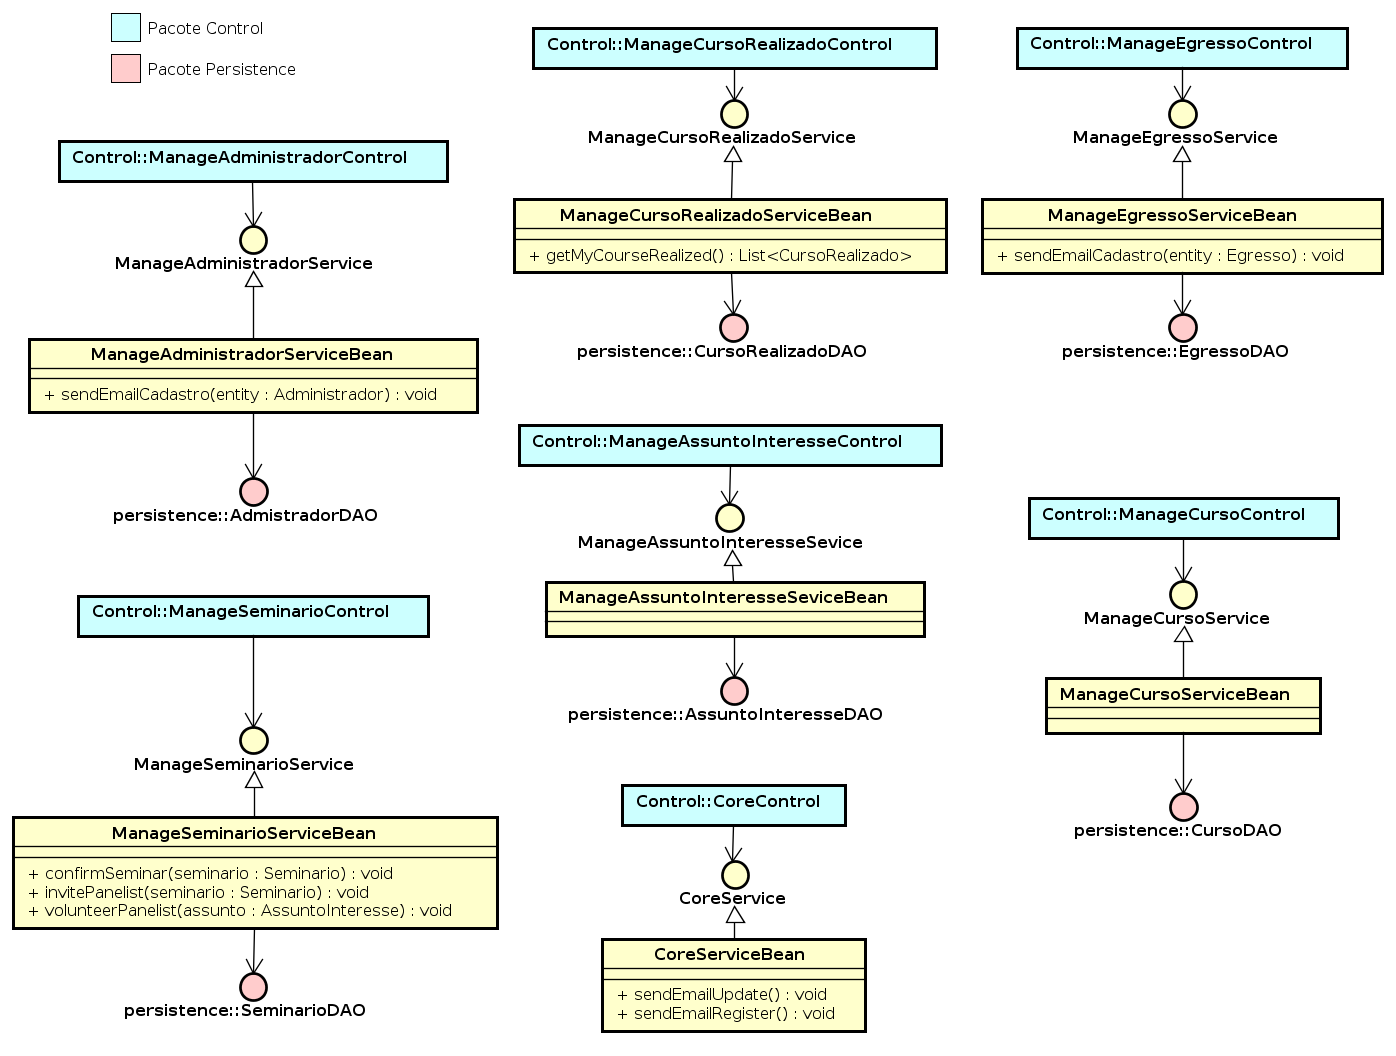
\includegraphics[width=1\textwidth]{figuras/modeloaplicacaocore.png}
  \caption{Modelo de Aplicação do SAE para o módulo \textit{sae.core}.}
  \label{figura-modelo-aplicacao-core}
\end{figure}

\begin{figure}[!h]
  \centering
  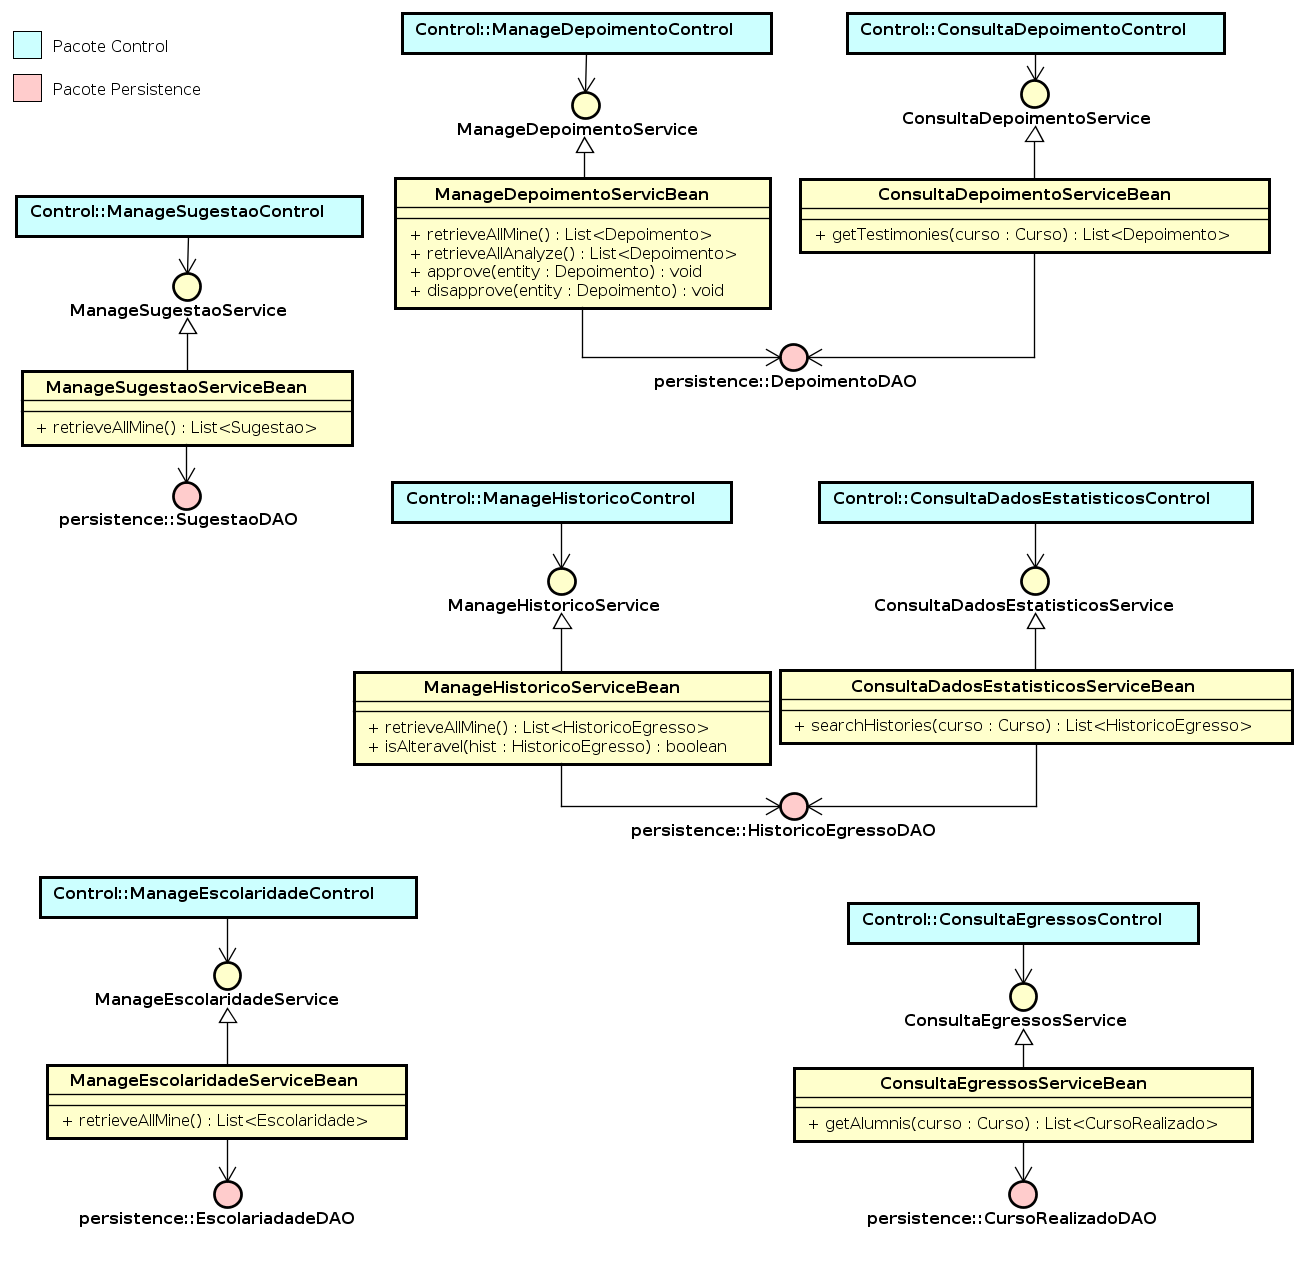
\includegraphics[width=1\textwidth]{figuras/modeloaplicacaopublico.png}
  \caption{Modelo de Aplicação do SAE para o módulo \textit{sae.public}.}
  \label{figura-modelo-aplicacao-publico}
\end{figure}

\newpage




%===================================================================================================================
%									Camada de Acesso a Dados
%===================================================================================================================
\section{Camada de Acesso a Dados}

Nesta seção são apresentados os Modelos de Persistência desenvolvidos para o projeto SAE e que foram usados na implementação do pacote de persistência.


Vale notar que o nome das classes já indica qual tecnologia de persistência foi utilizada, esse sistema de nomenclatura é mais uma sugestão do FrameWeb para simplificar o processo de software. Vale notar também que na Figura~\ref{figura-modelo-persistencia-generico} está representado o diagrama de persistência genérico provido pela ferramenta o nemo-utils. 




\begin{figure}[!h]
  \centering
  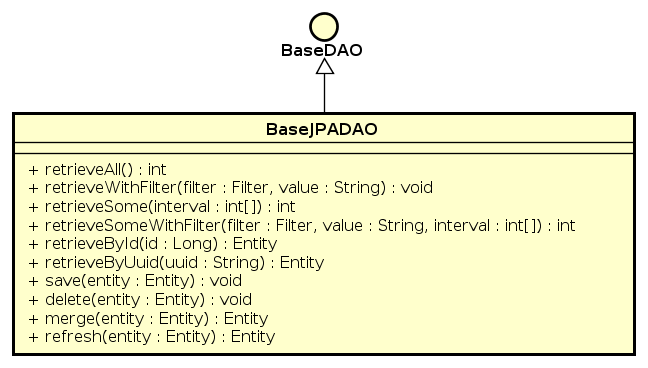
\includegraphics[scale=0.45]{figuras/baseJPADAO.png}
  \caption{Modelo de Persistência genérico da ferramenta nemo-utils.}
  \label{figura-modelo-persistencia-generico}
\end{figure}



Temos na Figura~\ref{figura-modelo-persistencia-core}  o modelo para o módulo \textit{sae.core} e na Figura~\ref{figura-modelo-persistencia-publico} o modelo para o módulo \textit{sae.public}.


\begin{figure}[!h]
  \centering
  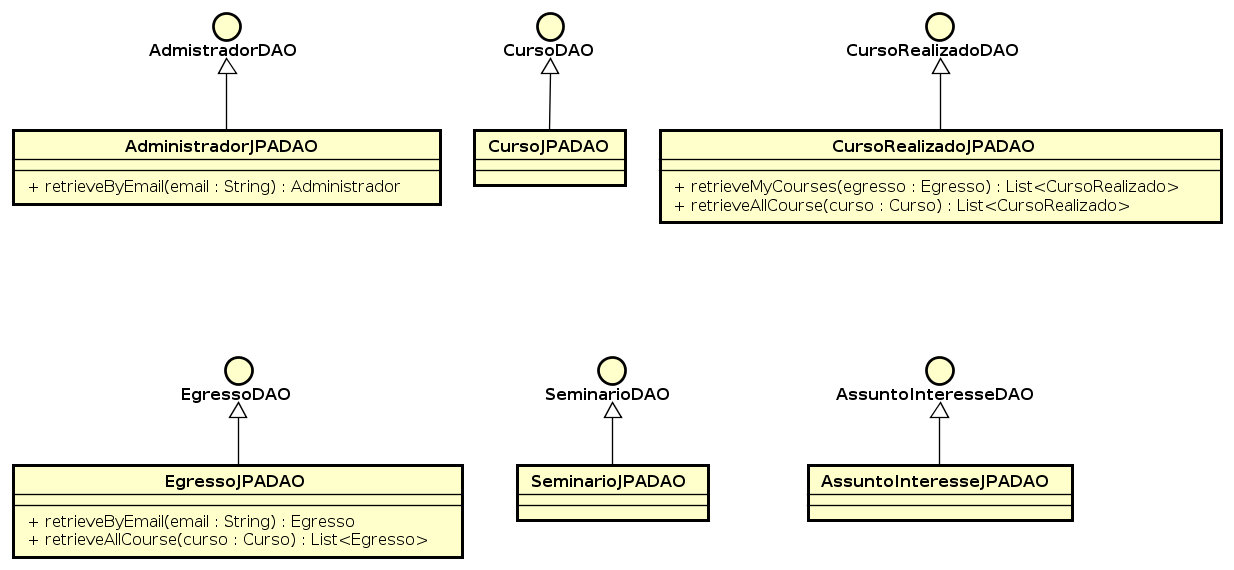
\includegraphics[width=1\textwidth]{figuras/modelopersistencecore.png}
  \caption{Modelo de Persistência do SAE para o módulo \textit{sae.core}.}
  \label{figura-modelo-persistencia-core}
\end{figure}

\newpage

\begin{figure}[!h]
  \centering
  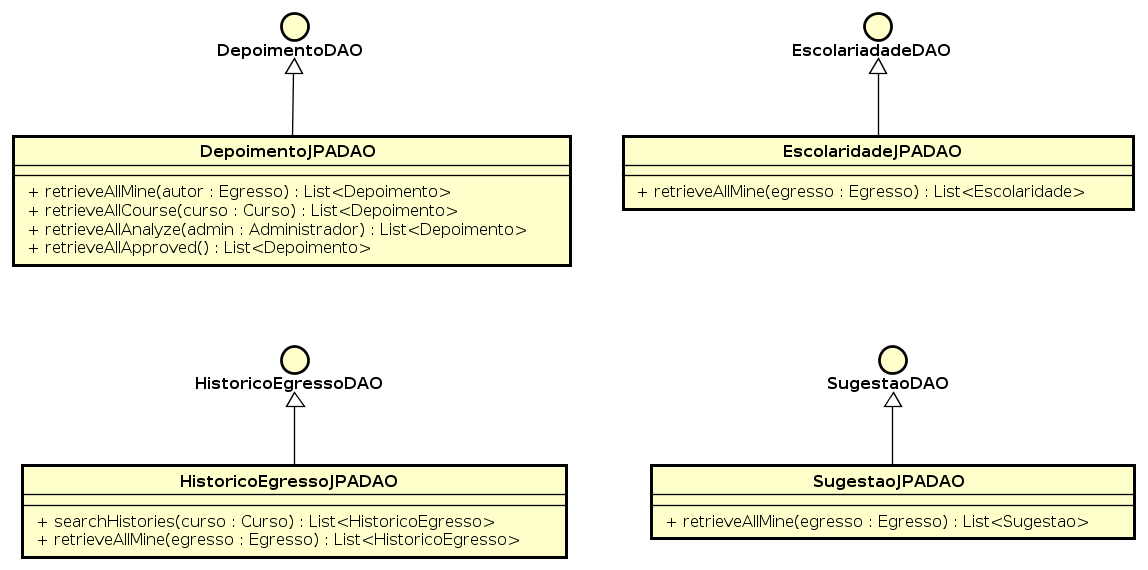
\includegraphics[width=1\textwidth]{figuras/modelopersistencepublico.png}
  \caption{Modelo de Persistência do SAE para o módulo \textit{sae.public}.}
  \label{figura-modelo-persistencia-publico}
\end{figure}




Note que a relação de herança entre os DAOs específicos e o DAO base não é representada explicitamente nos diagramas para evitar poluição visual. Esta também é uma recomendação do FrameWeb, ficando, portanto, o desenvolvedor incumbido de derivar essa relação implicitamente ao analisar o modelo.





%\include{capitulos/ch5-componentes}


%%% Páginas finais do documento: bibliografia e anexos. %%%
% Finaliza a parte no bookmark do PDF para que se inicie o bookmark na raiz e adiciona espaço de parte no sumário.
\phantompart

% Marca o início dos elementos pós-textuais.
\postextual

% Referências bibliográficas
\bibliography{bibliografia}

% Índice remissivo.
\phantompart
\printindex


\end{document}
